\documentclass[review,3p,authoryear]{elsarticle}

\usepackage[utf8]{inputenc}
\usepackage{amsmath,amssymb,amsthm}
\usepackage{mathtools}
\usepackage{booktabs}
\usepackage{longtable}
\usepackage{algorithm}
\usepackage{algpseudocode}
\usepackage{enumitem}
\usepackage{float}
\usepackage{graphicx}
\usepackage{pgfplots}
\pgfplotsset{compat=1.18}
\usepackage[hidelinks]{hyperref}
\pdfstringdefDisableCommands{%
  \def\corref#1{}%
  \def\cnotenum{}%
  \def\@corref#1{}%
}

% theorem environments
\theoremstyle{plain}
\newtheorem{theorem}{Theorem}
\newtheorem{proposition}{Proposition}
\newtheorem{lemma}{Lemma}
\theoremstyle{definition}
\newtheorem{definition}{Definition}
\newtheorem{example}{Example}
\theoremstyle{remark}
\newtheorem{remark}{Remark}

% notation shortcuts
\newcommand{\R}{\mathbb{R}}
\newcommand{\Rp}{\mathbb{R}_{\ge 0}}
\newcommand{\C}{\mathcal{C}}
\newcommand{\F}{\mathcal{F}}
\newcommand{\dom}{\operatorname{dom}}
\newcommand{\bp}{\operatorname{bp}}
\newcommand{\rc}{\bar{c}}
\newcommand{\Tmax}{T^{\max}}

\journal{Transportation Research Part B: Methodological}

\begin{document}

\begin{frontmatter}

\title{Branch-price-and-cut for the electric vehicle routing problem
with time windows, nonlinear charging and load-dependent discharging}

\author[tud]{Surendra Reddy Kancharla\corref{cor1}}
\ead{surendrareddy.kancharla@gmail.com}

\cortext[cor1]{Corresponding author}
\address[tud]{``Friedrich List'' Faculty of Transport and Traffic Sciences, Technische Universit\"at Dresden, Dresden, Germany}

\begin{abstract}
We study the electric vehicle routing problem (EVRP) with time windows, nonlinear
charging, and load-dependent discharging. This variant links routing,
payload-dependent energy use, partial recharging, and time feasibility, and has
previously been treated only by heuristic or compact mixed-integer programming
approaches on small instances. We propose a branch-price-and-cut algorithm whose
pricing problem is solved backward from the depot,
which makes the payload on every priced arc known when load-dependent energy is
evaluated. Nonlinear charging under time windows is represented by finite
piecewise-affine policies that map arrival charge and arrival time to continuation
cost and latest-arrival slack. We prove that the continuous station-extension
decision, including nested interactions among several charging stops, is exactly
captured by these policies. The set-partitioning master is strengthened by
decremental state-space relaxation, limited-memory subset-row cuts,
rounded-capacity cuts, customer-anchored branching, and a route-column disjunction
for residual fractional cases.
With exhaustive pricing the method proves optimality for the stated finite model;
budget-limited runs report certified bounds and status. On the tested benchmark
families, larger-cap audits return the same optima for all solved 10- and
20-customer instances. The algorithm proves all 10- and
20-customer instances in both the published load-dependent family and the generated
time-window family, proves several 40-customer instances, and improves on many
published load-dependent heuristic incumbents and MILP upper bounds.
\end{abstract}

\begin{keyword}
electric vehicle routing \sep nonlinear charging \sep load-dependent energy
consumption \sep branch-price-and-cut \sep column generation \sep function-valued
labeling
\end{keyword}

\end{frontmatter}

% ===========================================================================
\section{Introduction}
\label{sec:intro}

Routing a fleet of battery-electric vehicles is more than the classical vehicle
routing problem with relabeled cost coefficients. In the electric vehicle routing
problem (EVRP), limited range makes route construction and en-route recharging
inseparable. Vehicles must
be assigned not only to customers but also, when needed, to charging stations, and
those choices affect one another through both energy and time
\citep{SchneiderStengerGoeke2014}. A substantial literature has grown around this
interaction, progressively replacing early simplifying assumptions by more faithful
energy and charging models.

Two features are central in practical electric vehicle operation. Recharging is
nonlinear: A battery pack takes charge quickly when nearly empty and ever
more slowly as it fills, so the time required to reach a target charge is convex
and increasing. Discharging is load-dependent: The energy drawn per
kilometre grows with the payload, so a single consumption rate understates the
energy used on heavily loaded legs. Each feature is now well represented in the
literature when considered separately.

Their combination under time windows creates the main algorithmic difficulty. The
payload determines the energy consumed on an arc into a station; the resulting
arrival charge determines the feasible and useful departure charges; the departure
charge determines both downstream energy feasibility and charging time; and the
elapsed time must remain compatible with every downstream customer window and the
route horizon. The charging choice is therefore a trade-off between route cost and
future slack rather than a local minimum-time decision. An exact method must retain
that trade-off while also evaluating load-dependent energy exactly.

Exact optimization has addressed each feature separately but not their combination.
Branch-price-and-cut now reaches a hundred customers for nonlinear charging without
load dependence \citep{Nafstad2025,Lam2022}, and load-dependent transport
cost has been priced exactly in pickup-and-delivery routing
\citep{HasseIrnich2025}. The EVRP with nonlinear charging and
load-dependent discharging introduced by \citet{KancharlaRamadurai2020}, including
the time-window variants studied subsequently, has instead been solved by
heuristics or compact mixed-integer programming on small instances
\citep{KancharlaRamadurai2020,Xu2022,RastaniCatay2023,Yoshida2026}. To the best of
our knowledge, no exact algorithm has previously been published for the joint
nonlinear-charging, load-dependent-energy problem with time windows.

Our algorithm combines a backward pricer, which evaluates each load-dependent arc
with a known suffix payload, with finite cost--latest-arrival policies for the
continuous charging decision. The detailed construction is given in
Section~\ref{sec:bpc}.

We make four contributions. First, we give a set-partitioning formulation and an
exact branch-price-and-cut algorithm for the problem. Second, we develop a pricing
routine with exact load-dependent energy evaluation. Third, we
prove that the continuous station-extension problem has a finite piecewise-affine
representation, both for flat downstream continuations and for nested
station-over-tradeoff interactions. Fourth, we integrate the pricer into a complete exact framework with
dominance, decremental state-space relaxation, subset-row and rounded-capacity
cuts, customer-anchored branching, and a route-column disjunction for residual
fractional cases. We validate the implementation against an independent
continuous-charging reference and the
published load-dependent benchmark values of \citet{KancharlaRamadurai2020}.

The rest of the paper is organized as follows. Section~\ref{sec:lit} reviews the
literature on nonlinear charging, load dependence, and exact EVRP methods, and
locates our contribution within it. Section~\ref{sec:problem} defines
the problem and its set-partitioning model. Section~\ref{sec:bpc} develops the
algorithm, namely the pricer, the continuous-charging result, and
the dominance, relaxation, cutting, and branching around them. Section~\ref{sec:results}
reports the computational validation, and Section~\ref{sec:conclusion} concludes.

% ===========================================================================
\section{Related work}
\label{sec:lit}

The EVRP originates in green and alternative-fuel routing but departs from
it by treating recharging as a slow, en-route activity rather than a fixed
penalty. \citet{SchneiderStengerGoeke2014} formalized the version with time windows
and recharging stations under full, linear recharging, an early matheuristic for
which paired mixed-integer programming with variable-neighborhood search
\citep{bruglieri2015variable}; \citet{GoekeSchneider2015}
introduced a mixed conventional-electric fleet with a physically grounded energy
model. \citet{Desaulniers2016} then solved four time-window variants, single and
multiple, full and partial recharge, to optimality by branch-price-and-cut with
customized mono- and bidirectional labeling, reaching a hundred customers and
setting the template that later exact methods follow; the proliferation of variants
since is surveyed by \citet{ErdelicCaric2019} and \citet{kucukoglu2021electric}.

Nonlinear charging entered routing with \citet{Montoya2017}, who replaced the linear
refill with a concave state-of-charge curve, equivalently a convex
charging-time function, and contributed the piecewise-linear approximation
and the benchmark instances now standard in the field, solved there by a hybrid
metaheuristic. \citet{Froger2019} strengthened the formulations, showed the
path-based model to dominate node- and arc-based ones, and isolated the fixed-route
charging subproblem that recurs in later work; \citet{Bruni2025} encode the same
physics on a layered graph. Exact branch-price-and-cut for nonlinear charging
followed. \citet{lee2020exact} decomposed each route into maximum-range subpaths on
an extended charging-station network and priced them exactly, \citet{Liang2021}
priced the curve by recursion and
reached forty customers, \citet{Lam2022} added piecewise-linear recharging with
capacitated stations, and \citet{Nafstad2025} reached a hundred customers and
twenty-one stations with function-valued bidirectional labeling, with each label
carrying the whole map from arrival charge to best continuation, under heterogeneous
recharging technologies. A multiple-technology setting is also solved exactly by
the path-based branch-and-cut-and-price of \citet{Ceselli2021}, while
\citet{LeraRomero2024} carried exact pricing into the time-dependent setting. We adopt the same function-valued state; that representation is
not our contribution. What is new is making it carry load dependence.

Load dependence enters through the energy model of \citet{GoekeSchneider2015}, in
which consumption per unit distance is affine in gross weight, and through the
load-dependent cost problems built around it; \citet{kancharla2018adaptive} brought
weight-linear energy consumption into the EVRP with time windows under
adaptive large neighborhood search, and \citet{RastaniCatay2023} give a
large-neighborhood matheuristic for the load-dependent EVRP with time
windows. Its combination with nonlinear charging is exactly the E-VRP-NL-LD of
\citet{KancharlaRamadurai2020}, posed as a three-index arc model and solved by
adaptive large neighborhood search; \citet{Xu2022} extend the same combination to
simultaneous pickup and delivery, again heuristically, closing only small instances
with a commercial solver. Recent work has also addressed the hard-time-window
variant with a path-based formulation and ALNS \citep{Yoshida2026}. The joint
problem thus has no published exact algorithm to date, to the best of our
knowledge. The nearest exact result is \citet{HasseIrnich2025}, who price
load-dependent transport cost for pickup-and-delivery routing with time windows,
but with a cost linear in load and no nonlinear charging, so the two
nonlinearities never meet.

Two further lines refine EVRP inputs rather than the routing core. On the energy
side, the fidelity and uncertainty of the consumption
model have drawn sustained attention. \citet{basso2019energy} aggregate topography,
intersection stops, and acceleration into a physical driving-cycle estimate of
consumption, \citet{pelletier2019electric} hedge against consumption uncertainty
with a robust budgeted-deviation model solved by large neighborhood search and set
partitioning, and \citet{basso2021electric} pair Bayesian machine-learning energy
prediction with chance-constrained partial recharging. On the station side,
congestion and tariffs matter. \citet{keskin2019electric} model time-dependent
waiting at capacitated stations through an M/G/1 queue, and \citet{wang2026electric}
combine heterogeneous stations, time-dependent waiting, and time-of-use pricing.
These directions are largely orthogonal to ours. We hold a calibrated, deterministic
load-dependent energy model and a standard station model fixed in order to isolate
the exact treatment of nonlinear charging and load-dependent energy, and the pricer
developed here may be compatible with such refinements when they preserve the finite
piecewise-affine structure that the station-extension transform requires.

Methodologically we use the standard column-generation toolkit for routing, namely the
elementary resource-constrained shortest-path pricing problem
\citep{Feillet2004,IrnichDesaulniers2005}, the ng-route relaxation that contains
its combinatorics \citep{Baldacci2011}, subset-row
\citep{Jepsen2008,Pecin2017} and rounded-capacity
\citep{LysgaardLetchfordEglese2004} cuts, and dual stabilization
\citep{duMerle1999}. Bidirectional labeling \citep{RighiniSalani2006} is the
usual accelerator and underlies the hundred-customer results above, but
load-dependent energy makes its merge step less direct. We therefore use a purely
backward pricer and recover throughput through dominance, decremental state-space
relaxation, and parallelism. The continuous-charging characterization that follows
is, to our knowledge, new in either direction of labeling.

We position the contribution against the literature in Table~\ref{tab:positioning}.
Exact methods now reach nonlinear charging under time windows, and load-dependent
cost has an exact treatment, but the cell with nonlinear charging,
load-dependent energy, time windows, and an optimality guarantee was, before
this work, empty.

\begin{table}[t]
\centering
\caption{Positioning among exact EVRP methods.}
\label{tab:positioning}
\begin{tabular}{lcccc}
\toprule
 & NL & LD & TW & Exact \\
\midrule
\citet{Desaulniers2016}        & --         & --         & \checkmark & \checkmark \\
\citet{Montoya2017}            & \checkmark & --         & \checkmark & --         \\
\citet{lee2020exact}           & \checkmark & --         & --         & \checkmark \\
\citet{Froger2019}             & \checkmark & --         & \checkmark & \checkmark \\
\citet{Liang2021}              & \checkmark & --         & \checkmark & \checkmark \\
\citet{Lam2022}                & \checkmark & --         & \checkmark & \checkmark \\
\citet{Nafstad2025}            & \checkmark & --         & \checkmark & \checkmark \\
\citet{LeraRomero2024}         & \checkmark & --         & \checkmark & \checkmark \\
\citet{KancharlaRamadurai2020} & \checkmark & \checkmark & \checkmark & --         \\
\citet{RastaniCatay2023}       & \checkmark & \checkmark & \checkmark & --         \\
\citet{Xu2022}                 & \checkmark & \checkmark & \checkmark & --         \\
\citet{Yoshida2026}            & \checkmark & \checkmark & \checkmark & --         \\
\citet{HasseIrnich2025}        & --         & \checkmark$^{\dagger}$ & \checkmark & \checkmark \\
\textbf{This paper}            & \checkmark & \checkmark & \checkmark & \checkmark \\
\bottomrule
\end{tabular}
\vspace{2pt}
\begin{minipage}{0.98\linewidth}
\small
\emph{Notes.} NL: nonlinear charging; LD: load-dependent energy; TW: time
windows; Exact: proven optimality for the stated model under
exhaustive pricing. The dagger marks load-dependent cost rather than
energy.
\end{minipage}
\end{table}

% ===========================================================================
\section{Problem definition and set-partitioning model}
\label{sec:problem}

\subsection{Data and feasible routes}

Let \(G=(V,A)\) be a directed graph. The node set is
\(V=\{o,o'\}\cup\C\cup\F\), where \(\C\) is the customer set, \(\F\) is the
recharging-station set, and the depot is represented by a source \(o\) and an
identical sink \(o'\). Unless an instance excludes an arc, \(A\) contains every
ordered pair of distinct nodes that may be traversed. A homogeneous fleet of
electric vehicles, each with battery capacity \(Q\) (kWh) and freight capacity
\(W\) (kg), is based at the depot. Node coordinates induce Euclidean distances
\(d_{ij}\) for \((i,j)\in A\), and at a constant cruising speed the travel time on
arc \((i,j)\) is \(t_{ij}\). Each customer \(i\) has a demand \(q_i>0\), a service
time \(s_i\ge 0\), and a hard time window \([a_i,b_i]\). The vehicle may wait if it
arrives before \(a_i\) but may not arrive after \(b_i\). The depot window is
\([0,\Tmax]\), with \(\Tmax\) the route-duration horizon.

Two physical relations enter the model. On level terrain at fixed speed the energy
drawn on arc \((i,j)\in A\) with onboard payload \(u\) is affine in \(u\),
\begin{equation}
\label{eq:energy}
E_{ij}(u) \;=\; d_{ij}\,\bigl(\kappa^0 + \kappa^1 u\bigr),
\end{equation}
with an empty-vehicle rate $\kappa^0$ and a payload coefficient $\kappa^1$ that,
following \citet{KancharlaRamadurai2020}, depends only on rolling resistance and
drivetrain efficiency; $\kappa^1=0$ recovers the load-independent problem. Each
station $s\in\F$ has a cumulative charging-time function $\theta_s\colon[0,Q]\to\Rp$,
where $\theta_s(y)$ is the time to charge an empty battery to level \(y\); $\theta_s$
is continuous, nondecreasing, convex, and piecewise linear, with $\theta_s(0)=0$.
Convexity is the mathematical content of the tapering recharge rate. Recharging from
an arrival level $\alpha$ to a departure level $\beta\ge\alpha$ thus takes
\begin{equation}
\label{eq:chargecost}
\theta_s(\beta)-\theta_s(\alpha),
\end{equation}
and partial recharging is allowed, so $\beta$ is a continuous decision in
$[\alpha,Q]$. A station may be visited more than once on a route and, unlike a
customer, is not subject to a single-visit requirement; it carries an access window
$[a_s,b_s]$, which we take to be $[0,\Tmax]$ unless an instance restricts when the
station is open.

A route is an $o$--$o'$ walk that serves each of its customers exactly once,
interleaves station visits with departure-charge decisions, and is energy-, time-,
and capacity-feasible. The state of charge stays in $[0,Q]$ along the walk under the
consumption~\eqref{eq:energy} and charging~\eqref{eq:chargecost}, the vehicle
leaving $o$ fully charged; every customer is reached within its window and $o'$ by
$\Tmax$; and the served demand does not exceed $W$. Its cost is
\begin{equation}
\label{eq:routecost}
c_r \;=\; \sum_{(i,j)\in r} t_{ij} \;+\; \sum_{\text{recharges}}
\bigl(\theta_s(\beta)-\theta_s(\alpha)\bigr),
\end{equation}
the route's travel time plus its charging time. As in
\citet{Montoya2017}, waiting for a window to open consumes clock time but is not
charged in the objective; this is what lets time enter the route only through
feasibility, and is what makes a purely backward recursion well defined. A backward
label needs an upper bound on when it may arrive, not a forward accumulation
of elapsed time.

We solve the finite station-visit model. The number of station visits on a route is
bounded by a parameter \(\bar\sigma\). Such finite station-visit structure is common in
exact EVRP algorithms, appearing either explicitly through recharge-count
or station-copy limits \citep{SchneiderStengerGoeke2014,Desaulniers2016} or implicitly
through route-duration, elementarity, dominance, and finite path-state assumptions; the
bound is therefore not specific to our method. For the solved 10- and 20-customer
instances, Section~\ref{sec:results} further audits larger caps with four and five
station visits and verifies that the bound is nonbinding over that audited range.

\begin{table}[H]
\centering
% \setlength{\tabcolsep}{6pt}
\caption{Notation.}
\label{tab:notation}
% \small
\resizebox{0.7\textwidth}{!}{%
\begin{tabular}{@{}l p{0.62\linewidth}@{}}
\toprule
Symbol & Meaning \\
\midrule
\multicolumn{2}{@{}l}{\textit{Sets and indices}}\\
\(G=(V,A)\) & directed graph with node set \(V\) and arc set \(A\)\\
$\C,\ \F$ & customers; recharging stations\\
$o,\ o'$ & depot source and sink\\
$\Omega$ & set of feasible routes\\
$N_w$ & near-neighbor (\emph{ng}) memory set of customer $w$\\
\addlinespace[2pt]
\multicolumn{2}{@{}l}{\textit{Instance parameters}}\\
$Q,\ W$ & battery capacity (kWh); freight capacity (kg)\\
$d_{ij},\ t_{ij}$ & distance and travel time on arc $(i,j)$\\
$q_i,\ s_i,\ [a_i,b_i]$ & demand, service time, and time window of customer $i$\\
$\Tmax$ & route-duration horizon (depot window $[0,\Tmax]$)\\
$\kappa^0,\ \kappa^1$ & empty-vehicle and payload energy coefficients\\
$E_{ij}(u)$ & energy drawn on arc $(i,j)$ at payload $u$\\
$\theta_s(\cdot),\ [a_s,b_s]$ & charging-time function and access window of station $s$\\
$\bar\sigma$ & station-visit cap per route\\
\addlinespace[2pt]
\multicolumn{2}{@{}l}{\textit{Master problem and pricing}}\\
$x_r,\ c_r$ & route-selection variable; route cost\\
\(\nu_{ir}\) & number of times route \(r\) serves customer \(i\)\\
$\pi_i,\ \rc_r$ & dual of cover constraint $i$; reduced cost of route $r$\\
\addlinespace[2pt]
\multicolumn{2}{@{}l}{\textit{Backward label and policy} (\S\ref{sec:labeling})}\\
$P,\ k$ & backward partial path (route suffix) and its frontier node\\
$n_i(P)$ & suffix visits to customer $i$\\
$V(P),\ \sigma(P)$ & remembered customers (\emph{ng}-memory); station count\\
$\ell(P),\ \Pi(P)$ & suffix demand $\sum_i n_i(P)q_i$; suffix duals $\sum_i n_i(P)\pi_i$\\
$\mathcal P_P$ & finite policy set carried by the label\\
$p=(f_p,L_p^-,L_p^+,m_p,\rho_p)$ & cost--time tradeoff policy with cost function \(f_p\), latest-arrival band \(L_p^\pm\), slope \(m_p\), and ready floor \(\rho_p\)\\
$G_p,\ G_P$ & policy value; label value $\min_{p}G_p$ (lower envelope)\\
\(\Lambda_P\) & latest-arrival function for a flat continuation\\
\(\dom(f)\) & domain of function \(f\)\\
$\underline{y}_P,\ \overline{y}_P$ & smallest/largest arrival SOC in the policy domains\\
\addlinespace[2pt]
\multicolumn{2}{@{}l}{\textit{Continuous charging transform} (\S\ref{sec:continuous})}\\
$g$ & departure charge at a station (continuous decision)\\
$H(g),\ K(g)$ & cost key and clock-slack key of departure $g$\\
$I_j,\ d_j$ & charging pieces and their endpoints\\
$\Delta H_j,\ \Delta K_j$ & increments of $H,K$ across piece $I_j$\\
\bottomrule
\end{tabular}%
}
\end{table}

\subsection{Set-partitioning master}

Let $\Omega$ be the set of feasible routes and $\nu_{ir}$ the number of times route
$r$ serves customer $i$ (one for an elementary route). With binary variables $x_r$,
\begin{align}
\min \quad & \sum_{r\in\Omega} c_r\, x_r \label{eq:mp-obj}\\
\text{s.t.}\quad & \sum_{r\in\Omega} \nu_{ir}\, x_r = 1 && \forall\, i\in\C,
  \label{eq:mp-cover}\\
& x_r \in \{0,1\} && \forall\, r\in\Omega. \label{eq:mp-int}
\end{align}
The linear relaxation of the master~\eqref{eq:mp-obj}--\eqref{eq:mp-int}, restricted
to a manageable column pool, is solved by column
generation; let $\pi=(\pi_i)_{i\in\C}$ be the duals of \eqref{eq:mp-cover}. The
reduced cost of a route is $\rc_r = c_r - \sum_{i\in\C} \nu_{ir}\pi_i$, and pricing
seeks a feasible route of minimum reduced cost. If that minimum is nonnegative, the
restricted relaxation is optimal. Pricing is thus an elementary shortest-path
problem with resource constraints (ESPPRC), which is strongly NP-hard
\citep{Feillet2004}; we relax elementarity during pricing and restore it by
branching.
% ===========================================================================
\section{Branch-price-and-cut solution method}
\label{sec:bpc}

In outline the scheme is conventional. Each node of the branch-and-bound tree
solves the set-partitioning relaxation by column generation; the subproblem is the
backward labeling routine developed below, the node bound is sharpened by cutting
planes, and integrality is restored by branching. The search is best-first by node
bound with pruning against the incumbent, children warm-start from the parent's
column pool, and globally valid cuts are inherited. What makes the algorithm work
for this problem is not the outline but three of its parts, namely the backward pricer,
the treatment of continuous charging, and the dominance rule. We therefore develop
these three in detail and describe the standard machinery only as far as
correctness requires.

\subsection{Function-valued backward labeling}
\label{sec:labeling}

The pricer grows partial routes backward. A backward partial path $P$ is a feasible
walk from a frontier node $k$ to the sink $o'$; extending it means prepending
a node before $k$, moving the frontier one arc toward the source until the source
closes the route. The orientation is deliberate. If a backward suffix $P$ begins at
frontier $k$, and $n_i(P)$ is the number of suffix visits to customer $i$, then its
suffix demand is $ \ell(P)=\sum_{i\in\C} n_i(P)q_i .$

After the route departs a prepended node $w$ toward $k$, the vehicle still carries
exactly this multiset of suffix demands on the arc $(w,k)$. Thus the load-dependent
energy $E_{wk}(\ell(P))$ is known before the prefix is generated. For elementary
paths $n_i(P)\in\{0,1\}$; in the ng-route relaxation, repeated visits are treated
consistently as repeated relaxed services for load, reduced cost, and master-row
multiplicity.

The remaining state is the charge-time continuation. The charge with which the
vehicle arrives at the frontier is determined upstream and is unknown while $P$ is
processed, so the best completion of $P$ must be represented as a function of
arrival charge. Time windows add a cost-versus-slack trade-off, since extra charging
can improve downstream feasibility at the cost of recharge time. A label therefore
stores a finite policy set $\mathcal P_P$. Each policy $p\in\mathcal P_P$ is a coherent piecewise-affine
tradeoff with a ready-time floor $p=(f_p,L_p^-,L_p^+,m_p,\rho_p),~m_p\ge0,$
whose value at arrival charge \(y\) and arrival time \(\tau\) is $ G_p(y,\tau)=\widehat G_p(y,\max\{\tau,\rho_p\}),$
where
\[
\widehat G_p(y,\eta)=
\begin{cases}
f_p(y), & \eta\le L_p^-(y),\\
f_p(y)+m_p(\eta-L_p^-(y)), & L_p^-(y)<\eta\le L_p^+(y),\\
+\infty, & \eta>L_p^+(y).
\end{cases}
\]
Equivalently, a finite normalization can fold $\rho_p$ into the three
piecewise-affine functions by replacing $L_p^-$ with
$\max\{L_p^-,\rho_p\}$ on the feasible SOC domain and adding the corresponding
tradeoff penalty to $f_p$ where the floor lies inside the sloped band. The
implementation uses this finite breakpoint refinement to store normalized policies
with $\rho_p=0$. The label value is the lower envelope $G_P(y,\tau)=\min_{p\in\mathcal P_P}G_p(y,\tau). $

Flat continuations are the special case $m_p=0$ and $L_p^-=L_p^+$; when a label has
a single flat policy we write it as the pair $(f_P,\Lambda_P)$ for readability.
The functions within each policy refer to the same continuation, so latest
arrival and cost are never taken from different policies. By construction $G_P$ is
nonincreasing in \(y\). More arrival energy never makes the best continuation worse.
A node retains the set of non-dominated labels because a costlier policy set
that leaves more time slack can be the only continuation feasible upstream. The full
label
\begin{equation}
\label{eq:label}
\mathcal{L}(P) = \bigl(k,\,V(P),\,\sigma(P),\,\ell(P),\,\Pi(P),\,\mathcal P_P\bigr)
\end{equation}
also records the remembered visited customers $V(P)$ (elementary, or relaxed to an
\emph{ng}-memory as described shortly), the station count $\sigma(P)$, the suffix
demand $\ell(P)$, and the accumulated suffix duals
$\Pi(P)=\sum_{i\in\C}n_i(P)\pi_i$, with the same multiplicities as in $\ell(P)$.
Define
\[
\underline{y}_P=\min_{p\in\mathcal P_P}\min(\dom(f_p)),\qquad
\overline{y}_P=\max_{p\in\mathcal P_P}\max(\dom(f_p)).
\]
For \(y<\underline{y}_P\), the label value is \(+\infty\) because the arrival
charge is too small for any continuation. Above the last breakpoint at which a
represented continuation changes, surplus charge goes unused, so we adopt the
convention that each policy's cost and latest-arrival functions are defined on
the whole arrival-SOC interval up to \(Q\), extended as constants beyond that
saturation point; in particular \(\overline{y}_P=Q\). A policy is stored only on
the SOC subintervals where \(L_p^-(y)\le L_p^+(y)\); after any cap, ready-floor
normalization, or breakpoint refinement, subintervals violating this are discarded.
If such an operation leaves several disconnected SOC intervals, they are stored as
separate policies; hence each policy entering a station transform has an interval
domain.
The label and policy symbols are
collected with the rest of the notation in Table~\ref{tab:notation}.

The recursion starts at $o'$ with the singleton flat policy
$f\equiv0$, $L^-=L^+\equiv\Tmax$, $\rho=0$, and empty memory. Two extensions prepend
a node before $k$. Prepending a customer $w$ over the arc $(w,k)$, with arc energy
$E=E_{wk}(\ell(P))$, which is exact by the backward-load observation above, and
travel time $t=t_{wk}$, maps every downstream policy, after ready-floor
normalization, to
$p'=(f_{p'},L_{p'}^-,L_{p'}^+,m_p,a_w)$.
\begin{align}
f_{p'}(y) &= f_p(y-E) + t, & y &\in [\min(\dom(f_p))+E,\,Q],\label{eq:ref-cust-f}\\
L_{p'}^\pm(y) &= \min\{\,b_w,\ L_p^\pm(y-E)-s_w-t\,\}, &&\text{where } L_{p'}^+(y)\ge a_w,
  \label{eq:ref-cust-L}
\end{align}
with $\ell(P')=\ell(P)+q_w$, $\Pi(P')=\Pi(P)+\pi_w$, and a memory update
$V(P')=(V(P)\cap N_w)\cup\{w\}$ in which $N_w$ is a near-neighbor set whose role we
return to shortly. In the customer transform~\eqref{eq:ref-cust-f}--\eqref{eq:ref-cust-L},
the shift by $E$ is the energy drawn on the arc; the cap by $b_w$
and the floor at $a_w$ are the window. For a tradeoff policy, the customer child is
queried as $G_{p'}(y,\tau)=t+G_p(y-E,\max\{\tau,a_w\}+s_w+t)$, when the arrival at $w$ respects $b_w$ and is $+\infty$ otherwise; equivalently, the
implementation either stores $a_w$ as the policy's ready floor or normalizes it by
splitting/capping the piecewise-linear latest-arrival functions where that floor
or the due-date cap is met. Prepending a station $s^\star$ over
$(s^\star,k)$ applies the station
transform of Section~\ref{sec:continuous} to each $p\in\mathcal P_P$ and takes the
lower envelope of the emitted policies. The station's own access window
$[a_{s^\star},b_{s^\star}]$ enters the transform as a ready-time floor $a_{s^\star}$ and
a latest-arrival cap $b_{s^\star}$ on every emitted policy. In the
flat special case, with $E=E_{s^\star k}(\ell(P))$, $t=t_{s^\star k}$, and a
departure charge $g\in[E,Q]$, the vehicle arrives with charge \(y\le g\), charges to
$g$, and reaches $k$ with charge $g-E$; writing $\phi=f_P(g-E)$ and
$\lambda=\Lambda_P(g-E)$,
\begin{align}
f_{P'}(y) &= \bigl[\theta_{s^\star}(g)-\theta_{s^\star}(y)\bigr]+t+\phi,
  & y &\in[0,\,g],\label{eq:ref-stat-f}\\
\Lambda_{P'}(y) &= \min\{\,b_{s^\star},\ \theta_{s^\star}(y)+(\lambda-\theta_{s^\star}(g)-t)\,\},
  &&\text{where } \Lambda_{P'}(y)\ge a_{s^\star}.\label{eq:ref-stat-L}
\end{align}
Equations~\eqref{eq:ref-stat-f}--\eqref{eq:ref-stat-L} are the flat-policy nonlinear-charging transform. The recharge time depends on
both the unknown arrival charge \(y\) and the chosen departure \(g\), and the
\(-\theta_{s^\star}(y)\) term is what keeps the result a function of \(y\). One departure
deserves explicit mention. Charging nothing, \(g=y\), with the vehicle passing
through on the charge it arrives with, slides with \(y\) and so cannot be written as a
fixed-$g$ alternative; its value is
\begin{equation}
\label{eq:ref-stat-nc}
\begin{aligned}
f^{0}_{P'}(y)&=t+f_P(y-E),\\
\Lambda^{0}_{P'}(y)&=\min\{b_{s^\star},\ \Lambda_P(y-E)-t\},
\qquad y\in[\underline{y}_P+E,\,Q],
\end{aligned}
\end{equation}
feasible where $\Lambda^{0}_{P'}(y)\ge a_{s^\star}$, so the station access window is
enforced even when no energy is charged. This no-charge departure need not be generated
as a separate object: Theorem~\ref{thm:continuous} shows that the sliding choice \(g=y\)
is covered, or weakly dominated, by the same per-piece policies used for positive
charging. The route is closed
by prepending the source
$o$. The vehicle leaves fully charged and reaches $k$ with
$y_0=Q-E_{ok}(\ell(P))$ at time $t_{ok}$. Its reduced cost is $ t_{ok}+G_P(y_0,t_{ok})-\Pi(P),$ finite exactly when the source can complete the suffix.

\subsection{Exact pricing of continuous charging}
\label{sec:continuous}

The departure charge $g$ in the station extension is a continuous decision.
The implementation represents a downstream continuation by the finite policy set
introduced in Section~\ref{sec:labeling}. Each emitted policy is stored as
piecewise-affine functions $f,L^-,L^+$ over arrival state of charge, a slope $m$,
and a ready floor $\rho$; equivalently, one may normalize $\rho$ into the
piecewise-affine functions and split the policy into affine subpolicies at all
listed knots and floor crossings. Flat policies have $m=0$ and $L^-=L^+$. The
following theorem gives the flat transform, and
Theorem~\ref{thm:nested} gives the nested station-over-tradeoff composition used
when multiple charging stops interact through time windows.

Fix a station $s^\star$, frontier $k$, arc energy $E$, travel time $t$, and a flat
downstream policy $(f_P,\Lambda_P)$. For a departure charge $g$ define
\begin{equation}
\label{eq:keys}
H(g)=\theta_{s^\star}(g)+t+f_P(g-E),\qquad
K(g)=\Lambda_P(g-E)-\theta_{s^\star}(g)-t .
\end{equation}
For a station arrival charge \(y\le g\), the extension induced by \(g\) is
\[
f^{g}_{P'}(y)=H(g)-\theta_{s^\star}(y),\qquad
\Lambda^{g}_{P'}(y)=\min\{b_{s^\star},\,\theta_{s^\star}(y)+K(g)\}.
\]
Thus $H$ is the cost key and $K$ is the clock-slack key of the departure decision.

\begin{definition}[Charging pieces]
\label{def:cand}
Let $D=[d_0,d_m]$ with $d_0=\max\{E,\underline{y}_P+E\}$ and
$d_m=\min\{Q,\overline{y}_P+E\}$, where
$[\underline{y}_P,\overline{y}_P]=\dom(f_P)$. Set
\[
\mathcal{G}^\star=\Bigl[\bp(\theta_{s^\star})\cup(\bp(f_P)+E)\cup(\bp(\Lambda_P)+E)
\cup\{d_0,d_m\}\Bigr]\cap D,
\]
and list its elements as $d_0<d_1<\cdots<d_m$ (here $\bp(\cdot)$ denotes the breakpoint
set of a piecewise-linear function). The intervals
$I_j=[d_{j-1},d_j]$ are the charging pieces. On each $I_j$, both $H$ and $K$ are
affine. Under the domain convention of Section~\ref{sec:labeling} we have
$\overline{y}_P=Q$, so $d_m=Q$ and the pieces tile the entire feasible departure range
$[d_0,Q]$.
\end{definition}

\begin{theorem}[Exact flat-policy station extension]
\label{thm:continuous}
The continuous station extension is represented exactly by a finite set of
piecewise-affine policies. With the per-piece policies $G_j$ of the construction
below, the minimum over $j=1,\dots,m$ of $G_j(y,\tau)$ equals the continuous
station-extension optimum at every station arrival state $(y,\tau)$, with the departure
charge optimized continuously. The no-charge departure $g=y$ needs no separate policy:
it is covered by the same per-piece construction, either explicitly or by dominance
within a piece.
\end{theorem}

\paragraph{Construction of the per-piece policies.}
For each charging piece
$I_j=[d_{j-1},d_j]$, define
\(\xi_j(y)=\max\{y,d_{j-1}\}\) for \(y\in[0,d_j]\) and
\[
\Delta H_j=H(d_j)-H(d_{j-1}),\qquad
\Delta K_j=K(d_j)-K(d_{j-1}).
\]
The piece $I_j$ emits one
piecewise-affine tradeoff policy $(F_j,L_j^-,L_j^+,m_j)$, after refining the arrival
SOC domain by $\bp(\theta_{s^\star})\cup\{0,d_{j-1},d_j\}$, inserting any cap or
ready-floor crossing points, capping each latest-arrival function by $b_{s^\star}$,
and restricting to states with \(L_j^+(y)\ge a_{s^\star}\), as follows.
\[
\begin{array}{ll}
\Delta K_j>0,\ \Delta H_j>0:&
\begin{aligned}[t]
F_j(y)&=H(\xi_j(y))-\theta_{s^\star}(y),\\
L_j^-(y)&=\theta_{s^\star}(y)+K(\xi_j(y)),\\
L_j^+(y)&=\theta_{s^\star}(y)+K(d_j),\\
m_j&=\Delta H_j/\Delta K_j;
\end{aligned}\\[2mm]
\Delta K_j>0,\ \Delta H_j\le0:&
\begin{aligned}[t]
F_j(y)&=H(d_j)-\theta_{s^\star}(y),\\
L_j^-(y)&=L_j^+(y)=\theta_{s^\star}(y)+K(d_j),\\
m_j&=0;
\end{aligned}\\[2mm]
\Delta K_j<0,\ \Delta H_j<0:&
\begin{aligned}[t]
F_j(y)&=H(d_j)-\theta_{s^\star}(y),\\
L_j^-(y)&=\theta_{s^\star}(y)+K(d_j),\\
L_j^+(y)&=\theta_{s^\star}(y)+K(\xi_j(y)),\\
m_j&=\Delta H_j/\Delta K_j;
\end{aligned}\\[2mm]
\Delta K_j<0,\ \Delta H_j\ge0:&
\begin{aligned}[t]
F_j(y)&=H(\xi_j(y))-\theta_{s^\star}(y),\\
L_j^-(y)&=L_j^+(y)=\theta_{s^\star}(y)+K(\xi_j(y)),\\
m_j&=0;
\end{aligned}\\[2mm]
\Delta K_j=0:&
\begin{aligned}[t]
F_j(y)&=\min\{H(\xi_j(y)),H(d_j)\}-\theta_{s^\star}(y),\\
L_j^-(y)&=L_j^+(y)=\theta_{s^\star}(y)+K(d_{j-1}),\\
m_j&=0.
\end{aligned}
\end{array}
\]
For this policy, arrival at time \(\tau\) and charge \(y\) has value
\[
G_j(y,\tau)=
\begin{cases}
F_j(y), & \max\{\tau,a_{s^\star}\}\le L_j^-(y),\\
F_j(y)+m_j\bigl(\max\{\tau,a_{s^\star}\}-L_j^-(y)\bigr),
 & L_j^-(y)<\max\{\tau,a_{s^\star}\}\le L_j^+(y),\\
+\infty, & \max\{\tau,a_{s^\star}\}>L_j^+(y).
\end{cases}
\]

\begin{proof}
The breakpoint set in Definition~\ref{def:cand} contains every point at which
$\theta_{s^\star}$, $f_P(\cdot-E)$, or $\Lambda_P(\cdot-E)$ changes slope, so $H$ and
$K$ are affine on each $I_j$. The emitted arrival-SOC functions are then split at
the knots of $\theta_{s^\star}(y)$ and at $d_{j-1}$, so expressions such as
$H(d_{j-1})-\theta_{s^\star}(y)$ are never interpolated across a charging-curve
knot. Fix \(y\) and \(\tau\) and restrict the departure choice to one piece. Feasible
departures are \(g\in[\xi_j(y),d_j]\) satisfying
$\theta_{s^\star}(y)+K(g)\ge \max\{\tau,a_{s^\star}\}$,
and the value to minimize is \(H(g)-\theta_{s^\star}(y)\). This is a one-dimensional
linear program on an interval with at most one additional affine inequality.

Because $H$ and $K$ are affine on $I_j$, whenever $\Delta K_j\ne0$ we may eliminate $g$
and write $H$ as an affine function of $K$ with constant slope $\Delta H_j/\Delta K_j$;
one unit of additional latest-arrival slack therefore has constant marginal cost
$\Delta H_j/\Delta K_j$. The feasibility inequality
$\theta_{s^\star}(y)+K(g)\ge\max\{\tau,a_{s^\star}\}$ is nonbinding until the queried
latest arrival reaches the value associated with the least-cost feasible departure on
the piece, and is satisfiable up to the maximum latest-arrival value attainable on the
piece. Between these two thresholds the optimal value is affine with this marginal
slope; outside them it is either constant at the least-cost endpoint or infeasible.
This gives the stated two-threshold piecewise-affine form for $G_j$, whose base cost
$F_j$, lower and upper latest-arrival thresholds $L_j^-,L_j^+$, and slope $m_j$ are
read from the piece endpoints according to the sign of $(\Delta K_j,\Delta H_j)$: the
signs fix the least-cost endpoint and whether latest-arrival slack is gained by
increasing or decreasing $g$, which is exactly what the five rows of the construction
tabulate. (For instance, when both keys increase the least-cost departure is $\xi_j(y)$
and slack is bought up to $d_j$ at marginal cost $\Delta H_j/\Delta K_j$, the first row;
when $K$ increases but $H$ does not, $d_j$ dominates the piece and a flat policy
suffices, the second row.) The
cap at $b_{s^\star}$ is applied to both $L_j^-$ and $L_j^+$, and the ready-time floor
restricts the policy domain; capping a piecewise-linear latest-arrival function inserts
the crossing breakpoint when needed, so no slope break is lost, and the order
$L_j^-\le L_j^+$ is restored by discarding any subinterval where the cap inverts it.

The sliding no-charge departure \(g=y\) is covered by the same per-piece construction.
If \(y\in I_j\), then \(\xi_j(y)=y\). In the cases
\(\Delta K_j>0,\Delta H_j>0\) and \(\Delta K_j<0,\Delta H_j\ge0\), the emitted policy
uses \(\xi_j(y)\) as its base endpoint, so the no-charge value
\[
H(y)-\theta_{s^\star}(y)=t+f_P(y-E),\qquad
\theta_{s^\star}(y)+K(y)=\Lambda_P(y-E)-t
\]
appears directly, matching~\eqref{eq:ref-stat-nc} after the same latest-arrival cap is
applied. In the case \(\Delta K_j<0,\Delta H_j<0\), the uncapped policy recovers the
no-charge departure at the upper latest-arrival boundary of the tradeoff interval:
because \(H\) is affine in \(K\) on \(I_j\),
$ H(y)=H(d_j)+\frac{\Delta H_j}{\Delta K_j}\bigl(K(y)-K(d_j)\bigr),$
and evaluating the emitted policy at
\(L_j^+(y)=\theta_{s^\star}(y)+K(y)\) gives \(H(y)-\theta_{s^\star}(y)\). If the
due-time cap truncates this upper boundary, the retained domain requires no
latest-arrival value beyond the cap, and the same tradeoff policy has value no larger
than the no-charge value there. In the case \(\Delta K_j>0,\Delta H_j\le0\), departure
\(d_j\) weakly dominates \(g=y\), since it has cost no larger and provides at least as
large a latest-arrival value. When \(\Delta K_j=0\), the latest arrival is the same
throughout the piece and the policy retains the lower-cost choice among \(g=y\) and
\(g=d_j\). Thus no separate no-charge policy is required. Every fixed departure charge
lies in a charging piece, ties at shared piece endpoints may be assigned to either
adjacent piece without affecting the lower envelope, and the policy for that piece gives
the exact optimum of the restricted linear program. Taking the lower envelope over all
pieces gives the exact continuous station extension.
\end{proof}

\begin{example}[A two-piece station extension]
\label{ex:station}
Take $Q=10$ and a station whose charging-time function has two convex pieces,
$\theta_{s^\star}(y)=y$ on $[0,5]$ and $\theta_{s^\star}(y)=3y-10$ on $[5,10]$ (slopes
$1$ then $3$, with $\theta_{s^\star}(5)=5$). Let the downstream flat policy be
$f_P(y)=12-\tfrac12 y$ and $\Lambda_P(y)=8+2y$ on $[0,10]$, and set $E=t=0$ to isolate
the charging decision (nonzero $E,t$ only shift the arrival-SOC domain by $E$ and add
the constant $t$). The keys \eqref{eq:keys} are
\[
H(g)=\theta_{s^\star}(g)+12-\tfrac12 g,\qquad
K(g)=8+2g-\theta_{s^\star}(g),
\]
and the breakpoint set is $\mathcal G^\star=\{0,5,10\}$, giving pieces $I_1=[0,5]$ and
$I_2=[5,10]$.

On $I_1$ one has $H(g)=12+\tfrac12 g$ and $K(g)=8+g$, so $\Delta H_1=2.5>0$ and
$\Delta K_1=5>0$, giving the tradeoff case with slope $m_1=\Delta H_1/\Delta K_1=\tfrac12$ and,
using \(\xi_1(y)=y\),
\[
F_1(y)=H(y)-\theta_{s^\star}(y),\quad
L_1^-(y)=\theta_{s^\star}(y)+K(y),\quad
L_1^+(y)=\theta_{s^\star}(y)+K(5).
\]
Charging past the arrival charge increases latest-arrival slack up to $g=5$ at price
$\tfrac12$ per unit. On $I_2$ one has $H(g)=\tfrac52 g+2$ and $K(g)=18-g$, so
$\Delta H_2=12.5>0$ while $\Delta K_2=-5<0$. Charging into $[5,10]$ costs more
and removes slack, so the left feasible endpoint
\(\xi_2(y)=\max\{y,5\}\) dominates. The piece emits the flat policy
\[
F_2(y)=H(\xi_2(y))-\theta_{s^\star}(y),\qquad
L_2^\pm(y)=\theta_{s^\star}(y)+K(\xi_2(y)).
\]
For the plotted arrival \(y=2\), this reduces to
\(F_2(2)=H(5)-\theta_{s^\star}(2)\) and
\(L_2^\pm(2)=\theta_{s^\star}(2)+K(5)\). For this plotted arrival, the no-charge
departure \(g=y\) needs no separate policy: its value~\eqref{eq:ref-stat-nc}
\(f^0(2)=f_P(2)\), \(\Lambda^0(2)=\Lambda_P(2)\) coincides with the base of the \(I_1\) policy,
illustrating the subsumption used in the proof of Theorem~\ref{thm:continuous}.

At arrival charge \(y=2\) (so \(\theta_{s^\star}(2)=2\)) this gives $F_1(2)=11$,
$L_1^-(2)=12$, $L_1^+(2)=15$, and the $I_2$ policy value $12.5$ at latest arrival $15$,
so the lower envelope is
\[
G(2,\tau)=
\begin{cases}
11, & \tau\le 12,\\
11+\tfrac12(\tau-12), & 12<\tau\le 15,\\
+\infty, & \tau>15.
\end{cases}
\]
Thus the envelope selects no additional charge when the downstream window is loose,
increases the departure charge along $I_1$ as the time constraint tightens, and becomes
infeasible once charging to $g=5$ still cannot meet $\tau$. The two
pieces and their lower envelope are exactly the objects of
Theorem~\ref{thm:continuous}, with the no-charge departure appearing as the least-cost
endpoint of $I_1$; Figure~\ref{fig:example} plots $\theta_{s^\star}$ and the
resulting envelope $G(2,\tau)$.
\end{example}

\begin{figure}[H]
\centering
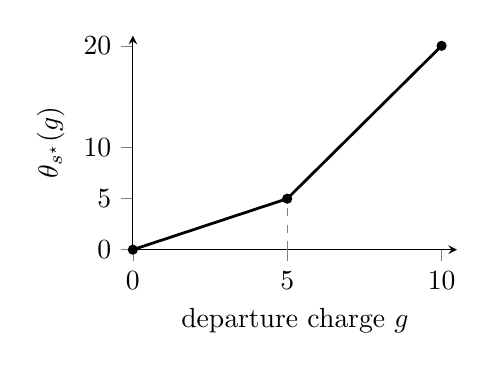
\begin{tikzpicture}
\begin{axis}[
  width=0.47\linewidth, height=4.3cm,
  axis lines=left, tick align=outside,
  xlabel={departure charge $g$}, ylabel={$\theta_{s^\star}(g)$},
  xmin=0, xmax=10.5, ymin=0, ymax=21,
  xtick={0,5,10}, ytick={0,5,10,20},
  every axis plot/.append style={line width=1pt},
]
\addplot[black, mark=*, mark size=1.3pt] coordinates {(0,0) (5,5) (10,20)};
\draw[dashed, gray] (axis cs:5,0) -- (axis cs:5,5);
\end{axis}
\end{tikzpicture}\hfill
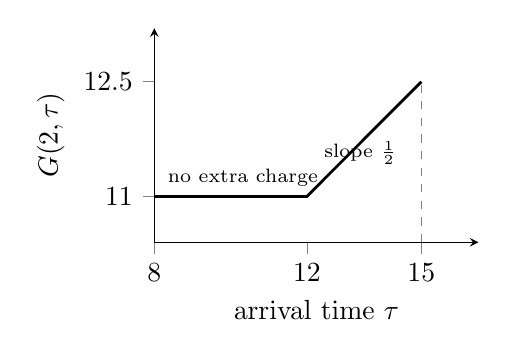
\begin{tikzpicture}
\begin{axis}[
  width=0.47\linewidth, height=4.3cm,
  axis lines=left, tick align=outside,
  xlabel={arrival time $\tau$}, ylabel={$G(2,\tau)$},
  xmin=8, xmax=16.5, ymin=10.4, ymax=13.2,
  xtick={8,12,15}, ytick={11,12.5},
  every axis plot/.append style={line width=1pt},
]
\addplot[black] coordinates {(8,11) (12,11) (15,12.5)};
\draw[dashed, gray] (axis cs:15,10.4) -- (axis cs:15,12.5);
\node[anchor=south west, font=\scriptsize] at (axis cs:8.1,11) {no extra charge};
\node[anchor=north west, font=\scriptsize] at (axis cs:12.2,11.85) {slope $\tfrac12$};
\end{axis}
\end{tikzpicture}
\caption{Example~\ref{ex:station}: the two-segment charging curve $\theta_{s^\star}$
(left, breakpoint at $g=5$) and the resulting best-continuation cost $G(2,\tau)$ at
arrival charge \(y=2\) (right). For $\tau\le 12$ the least-cost departure adds no charge
(cost $11$); for $12<\tau\le 15$ charging along piece $I_1$ increases latest-arrival
slack at slope $\tfrac12$; for $\tau>15$ no departure is feasible.}
\label{fig:example}
\end{figure}

\begin{theorem}[Nested station-over-tradeoff extension]
\label{thm:nested}
A downstream cost--time tradeoff is also represented exactly by finitely many
policies. After capping latest-arrival functions by $b_{s^\star}$ and applying the
ready-time floor at $s^\star$, the lower envelope of the policy families built below
equals the continuous station-extension optimum at every arrival state, and applying
this independently to every downstream policy gives an exact finite representation
for arbitrary multi-station chains. Let the downstream continuation contain a tradeoff policy
$p=(f,L^-,L^+,m,\rho)$ with $m>0$, normalized so that $\rho=0$. On a common affine departure interval
$I_j=[d_{j-1},d_j]$ for
$\theta_{s^\star}$, $f(\cdot-E)$, $L^-(\cdot-E)$, and $L^+(\cdot-E)$, define
\[
H(g)=\theta_{s^\star}(g)+t+f(g-E),\quad
K^-(g)=L^-(g-E)-\theta_{s^\star}(g)-t,\quad
K^+(g)=L^+(g-E)-\theta_{s^\star}(g)-t,
\]
and
\[
\bar H(g)=H(g)+m\bigl(K^+(g)-K^-(g)\bigr)
          =\theta_{s^\star}(g)+t+f(g-E)+m\bigl(L^+(g-E)-L^-(g-E)\bigr).
\]
The transform emits, over all common intervals, the following finite policy
families:

\begin{enumerate}[label=(\roman*)]
\item the flat-policy transform of Theorem~\ref{thm:continuous} applied to
$(H,K^-)$, representing arrivals that remain on the base part of $p$;
\item the same transform applied to $(\bar H,K^+)$, representing arrivals at
the high-latest boundary of $p$;
\item the interior-departure families: for each interval endpoint selector
\(e_j(y)\in\{\max\{y,d_{j-1}\},d_j\}\),
the tradeoff policy
\[
\begin{aligned}
F_j^e(y)&=H(e_j(y))-\theta_{s^\star}(y),\\
L_{j}^{e,-}(y)&=\theta_{s^\star}(y)+K^-(e_j(y)),\\
L_{j}^{e,+}(y)&=\theta_{s^\star}(y)+K^+(e_j(y)),\\
m_j^e&=m .
\end{aligned}
\]
\end{enumerate}
\end{theorem}

\begin{proof}
Fix \(y\), set \(\eta=\max\{\tau,a_{s^\star}\}\), and write
\(u=\eta-\theta_{s^\star}(y)\). For a fixed departure \(g\), the downstream policy contributes
\[
H(g)-\theta_{s^\star}(y)
\]
when $u\le K^-(g)$, contributes
\[
H(g)-\theta_{s^\star}(y)+m(u-K^-(g))
\]
when $K^-(g)<u\le K^+(g)$, and is infeasible when $u>K^+(g)$. Thus the minimization
over \(g\in[\max\{y,d_{j-1}\},d_j]\) is a one-dimensional piecewise-linear program.
If the optimum is on the base boundary $u\le K^-(g)$, it is represented by the flat
transform over $(H,K^-)$. If it is on the high-latest boundary $u=K^+(g)$, substituting
$u=K^+(g)$ gives the cost key $\bar H(g)$ and the flat transform over $(\bar H,K^+)$.
This transform represents optima on that boundary; for $u<K^+(g)$ it may overestimate
the value of the same departure but never underestimates it, so its inclusion in the
lower envelope cannot reduce the computed value below the restricted optimum. When the
restricted optimum lies on \(u=K^+(g)\), the corresponding departure is included with
its exact value. Otherwise consider the interior tradeoff region \(K^-(g)<u<K^+(g)\),
where the value is
$ \bigl(H(g)-m\,K^-(g)\bigr)+m\,u-\theta_{s^\star}(y),$ which is affine in \(g\) for fixed \(u\). Over the closure of
$ \{g:K^-(g)<u<K^+(g)\}\cap[\max\{y,d_{j-1}\},d_j],$
an affine function attains its minimum at an endpoint. If that endpoint is one of the
original interval endpoints \(\max\{y,d_{j-1}\}\) or \(d_j\), it is represented by the
fixed-departure policies in (iii). If the endpoint satisfies \(K^-(g)=u\), it is
represented by the flat transform over \((H,K^-)\) in (i); if it satisfies \(K^+(g)=u\),
it is represented by the transform over \((\bar H,K^+)\) in (ii). Hence at least one
emitted family attains the optimum of the restricted one-dimensional program. The
breakpoint set contains all slope changes of the four functions, so the argument applies
on every common affine interval; the lower envelope over intervals and downstream
policies is therefore exact.
\end{proof}

The policy class is closed under the two extensions in the finite sense needed by
the pricer. A customer extension shifts SOC knots by the arc energy, shifts and
caps latest-arrival functions by service, travel time, and the customer due time,
and normalizes the ready floor; this inserts only finitely many crossing knots. A
station extension forms common affine departure intervals from the finite union of
charging-curve knots and shifted knots of $f,L^-,L^+$, and
Theorems~\ref{thm:continuous} and~\ref{thm:nested} emit finitely many policy
families on each interval. Keeping the lower envelope
as a finite list of emitted policies and inducting over the finite sequence of
admissible extensions gives a finite representation for every backward partial path.

\begin{remark}
The flat theorem is deliberately stronger than a breakpoint enumeration. In the two
tradeoff cases, the optimal departure can lie in the interior of $I_j$ at the point
where the slack inequality binds, and that point depends on the queried arrival time
$\tau$. The nested theorem shows that a downstream cost-versus-time slope preserves
finiteness; it adds the high-latest boundary and the two fixed-departure
families. Both proofs use only that $\theta_{s^\star}$, $f_P$, and $\Lambda_P$ are
piecewise-linear; convexity of $\theta_{s^\star}$, the tapering recharge rate assumed in
the charging model, is a property of the instances rather than a hypothesis of the
theorems, which hold for any piecewise-linear charging-time curve. The implementation
validates these emitted policy sets against an
independent direct evaluator, including downstream ready-time waiting. That
reference enumerates elementary customer orders and station insertions on small
instances and solves the continuous charging/time-window problem for each fixed
path independently; validation compares reduced costs and reconstructed charging
schedules within numerical tolerance.
\end{remark}

\subsection{Dominance}
\label{sec:dominance}

Labels are pruned by the standard dominance argument, made to respect the functional
resources. The two extensions are isotone in the label value, which establishes the
soundness of the rule below.

\begin{lemma}[Monotonicity of the extensions]
\label{lem:monotone}
Suppose $G_P\le G_{P'}$ at every arrival state where $G_{P'}$ is finite. Then after either
a customer or a station extension by the same arc, the resulting children $Q,Q'$ satisfy
$G_Q\le G_{Q'}$ wherever $G_{Q'}$ is finite.
\end{lemma}

\begin{proof}
The customer transform~\eqref{eq:ref-cust-f}--\eqref{eq:ref-cust-L} composes $G_P$ with an
affine shift of its arguments and adds the constant travel time, so it preserves the
pointwise order. The station transform takes, at each arrival $(y,\tau)$, a minimum over
feasible departures $g$, with $\eta=\max\{\tau,a_{s^\star}\}$, of
\[
\theta_{s^\star}(g)-\theta_{s^\star}(y)+t
+G_P\bigl(g-E,\eta+\theta_{s^\star}(g)-\theta_{s^\star}(y)+t\bigr).
\]
Using the pointwise no-larger value function $G_P$ in place of $G_{P'}$ cannot increase
the minimand at any $g$, and therefore cannot increase the minimum. Lower envelopes preserve
the order, so $G_Q\le G_{Q'}$.
\end{proof}

\begin{proposition}[Dominance]
\label{prop:dominance}
Let $P,\tilde P$ share a frontier. Suppose $V(P)\subseteq V(\tilde P)$,
$\sigma(P)\le\sigma(\tilde P)$, $\ell(P)\le\ell(\tilde P)$,
$\underline{y}_P\le\underline{y}_{\tilde P}$, and, for every arrival state
$(y,\tau)$ for which $G_{\tilde P}(y,\tau)<+\infty$,
\[
G_P(y,\tau)-\Pi(P)\ \le\ G_{\tilde P}(y,\tau)-\Pi(\tilde P).
\]
Then $P$ dominates $\tilde P$. Every feasible completion of $\tilde P$ has a
corresponding completion of $P$ with no greater reduced cost, so $\tilde P$ may be
discarded.
\end{proposition}

\begin{proof}
Any prefix $R$ completing $\tilde P$ and reaching its frontier at time $\tau_0$
also completes $P$. It uses no customer of
$V(\tilde P)\supseteq V(P)$, adds the same station visits to both, and, because
$\ell(P)\le\ell(\tilde P)$, keeps the total demand within $W$. Since $P$ carries no
more suffix load, $R$ draws no more energy on the prefix, so the route built on $P$
reaches the frontier with at least as much charge \(y_0^P\ge y_0^{\tilde P}\). As
$G_P$ is nonincreasing in state of charge and
\(y_0^{\tilde P}\ge\underline{y}_{\tilde P}\ge\underline{y}_P\), the value inequality
at the common arrival time $\tau_0$ gives
\[
G_P(y_0^P,\tau_0)-\Pi(P)
\le
G_{\tilde P}(y_0^{\tilde P},\tau_0)-\Pi(\tilde P),
\]
and the common prefix cost cancels. If \(G_{\tilde P}(y_0^{\tilde P},\tau_0)\) is
finite, then \(G_P(y_0^P,\tau_0)\) is finite as well, so time feasibility is preserved.
By Lemma~\ref{lem:monotone} the same comparison holds when $R$ is applied one arc at a
time rather than at once, so the dominance is preserved throughout the extension.
\end{proof}

The proposition states the exact dominance criterion as a pointwise inequality between
the two labels' lower envelopes $G_P$ and $G_{\tilde P}$. Checking that envelope
inequality directly is computationally inconvenient, because each envelope is itself a
minimum over its policies; the implementation therefore certifies a sufficient condition that
implies it. Every policy of the dominated label $\tilde P$ is pointwise dominated by a
single policy of the candidate $P$. Since $G_P$ is the lower envelope of its
policies, this per-policy covering forces $G_P\le G_{\tilde P}$ at every arrival state,
so the hypothesis of Proposition~\ref{prop:dominance} holds and the discard is valid.
For a policy pair, the SOC axis is refined at all breakpoints of $f,L^-,L^+$ and at
every intersection of the ready-time, $L^-$, and $L^+$ boundary lines of the two
policies; on each resulting cell both policy values are affine in $(y,\tau)$, so a
non-strict inequality at the cell vertices proves dominance on that cell. The
certificate is therefore a conservative sufficient test for the proposition. It may
miss a dominance that holds only for the combined envelope, where several policies of
$P$ jointly cover one policy of $\tilde P$, but it never discards a label the exact
criterion would keep. It licenses comparing a whole batch of new labels against the
current frontier in parallel and reconciling them in sequence, with the optimum
untouched.
The load and least-feasible-charge conditions are coordinatewise, so labels may be
bucketed along those two axes and each compared only against buckets that can
possibly dominate it.

\subsection{Decremental state-space relaxation}
\label{sec:relax}

Full elementarity makes the label space unmanageable, so we price over the
\emph{ng}-route relaxation with decrementally grown memories
\citep{Baldacci2011,RighiniSalani2006}: pricing at the root starts from empty memories,
and each child inherits the parent's critical set as a warm start. Whenever the returned
route repeats a customer, that customer is added to the local
critical set $\Sigma$ that every memory must thereafter contain and the node is
repriced, until the minimum-reduced-cost route is elementary. Since $\Sigma$ only grows
and is bounded by $\C$, the loop terminates. Two points are specific to this problem.
First, validity of the bound requires
that the coverage coefficient $\nu_{ir}$ count multiplicity: a route serving a
customer twice contributes a $2$ to that partition row, which the row at value one
cannot accept, so non-elementary columns enter only fractionally and never falsify the
bound. The master therefore remains the current ng relaxation and supplies a valid lower
bound rather than a solved full-elementary LP; when $\Sigma$ grows, any restricted-master
column revisiting a now-critical customer is removed before the node LP is used as a
proof bound, while remaining ng-feasible columns are still charged by multiplicity and
their cut states tracked by the same per-route counters, so cut pricing stays consistent.
Second, convergence is certified by an exact threshold predicate rather than the full
minimum reduced cost: the pricer is asked only whether a route below a small negative
tolerance exists, a negative answer certifying the node (the current relaxation contains
every elementary route) and a positive answer triggering a normal sweep that adds columns
or tightens a memory. This lets the backward search stop as soon as the threshold is
crossed.

\subsection{Valid inequalities}
\label{sec:cuts}

Two families of cuts tighten the node bound. The first are limited-memory subset-row
inequalities \citep{Jepsen2008,Pecin2017}. For an odd customer set $U$ (we separate
triplets), the inequality
\[
\sum_{r}\left\lfloor\tfrac12\sum_{i\in U}\nu_{ir}\right\rfloor x_r
\le \left\lfloor |U|/2\right\rfloor
\]
is a rank-one rounding of the partition rows, with dual $\gamma_U\le0$, priced as a
penalty $\gamma_U$ charged the second time a route enters $U$ and tracked by a per-cut
label counter. As the penalty makes the suffix cost counter-dependent, dominance is made
conservative in the standard manner \citep{Jepsen2008}: when a candidate label
P has entered more of $U$ than a comparator \(\tilde{P}\), the
nonnegative amount $ -\gamma_U\left\lceil\tfrac12
\bigl(n_U(P)-n_U(\tilde{P})\bigr)^+\right\rceil $
is added to the candidate's cost before comparison, which only over-charges it and so
cannot discard a needed label.

The second are rounded-capacity inequalities in route-count form
\citep{LysgaardLetchfordEglese2004}. For a customer set $U$ of total demand $d(U)$,
\begin{equation}
\label{eq:rcc}
\sum_{r:\ \mathrm{supp}(r)\cap U\ne\varnothing} x_r \;\ge\; \bigl\lceil d(U)/W \bigr\rceil,
\end{equation}
which holds because the routes meeting $U$ must between them carry all of $d(U)$ and
each carries at most $W$. The dual is a reward earned once when a route first enters
$U$, priced by a one-shot bonus and a one-bit flag, with the same conservative one-sided
dominance correction as above but sign-reversed: a reward the candidate has claimed and
the comparator has not is added back to the candidate before comparison, again weakening
dominance only and so never pruning an improving route.

\subsection{Branching and integer optimality}
\label{sec:branching}

From a fractional solution we first try customer-anchored arc branching,
aggregating flow on arcs incident to a customer: a fractional arc creates a child that
forbids it and a child that forces it as the customer endpoint's unique predecessor or
successor, both passed to pricing as forbidden-arc sets. Station arcs are not forced,
since stations are revisitable. If all customer-incident arcs are integral, residual
fractionality can still arise from station or charging differences among columns sharing
a customer projection. We retain only the least-cost representative among columns with
identical full master-column vectors; if two remaining positive columns differ in
customer support, standard Ryan--Foster branching on a pair $(i,j)$ with
$0<\sum_{r''\ni i,j}x_{r''}<1$ requires or forbids the pair to share a route.

If fractionality remains only within identical customer-support classes, we branch on an
exact route signature -- the ordered depot, customer, and station visits together with
the induced full master-column vector. The $x_r=0$ child bans that signature. The
$x_r=1$ child fixes the column,
subtracts its coefficients from all residual rows, and restricts residual pricing to
routes disjoint from its customers; if the fixed column repeats a customer, this child
is infeasible. For a fixed signature the exact evaluator inserts only the minimum-cost
column over continuous charging decisions, so the column is well defined. This finite
disjunction, together with customer-anchored arc branching, separates every fractional
node.

Each node relaxation remains a set-partitioning LP. One artificial variable per
customer keeps the restricted master feasible and its duals usable for pricing; a node
is declared infeasible only after pricing certifies that no negative-reduced-cost
column can remove an active artificial. We do not use a covering relaxation: overlapping
routes can cover every customer while serving some customer more than once, yielding a
bound below the partitioning bound and invalid pruning.

% ===========================================================================
\section{Computational experiments}
\label{sec:results}

\subsection{Benchmark sets and protocol}
We use the following naming convention. E-VRP-NL denotes the EVRP with nonlinear
charging, E-VRP-NL-LD adds load-dependent discharging, and E-VRPTW-NL-LD further
adds customer time windows. We evaluate the algorithm on two load-dependent benchmark
families. The first, E-VRP-NL-LD, is the family without time windows, using the
demands and load-dependent energy coefficients of \citet{KancharlaRamadurai2020}.
The second, E-VRPTW-NL-LD, adds generated feasible customer time windows to the same
load-dependent instances, and is the principal test for the
cost--latest-arrival policies. The family with time windows is generated for this
study and has no published best-known
values; the exact generated instance files are part of the benchmark archive and
future regeneration uses deterministic per-file seeds. The benchmark archive is
available at \url{https://t.ly/tLYCY}. Both families are reported by their bounds and
incumbents.

All objectives are travel plus charging time in hours, matching the published
objective. The runs use the native
per-instance energy calibration, the continuous exact station-extension backend,
state-of-charge bucketing, decremental state-space relaxation, and a station-visit
cap \(\bar\sigma=3\). Table~\ref{tab:cap-sensitivity} audits this cap on the
solved 10- and 20-customer instances. Each instance is solved independently on a
single thread under a three-hour per-instance time
budget checked between pricing operations, so a final sweep can carry the reported
wall time a few seconds beyond 10800 seconds. All experiments were conducted on an Intel Core i9-14900K
processor at 5.6\,GHz with 128\,GB of RAM running Ubuntu 24.04. When pricing
exhausts the search space, the reported lower bound is valid; optimality is
certified when that bound equals the incumbent. If a run stops during pricing, the
incumbent remains a feasible upper bound but no final gap is available.

\subsection{Aggregate performance}
Table~\ref{tab:bench-summary} summarizes the complete run. The
E-VRP-NL-LD instances without time windows are solved to proven optimality for all
10- and 20-customer cases and for three of the 40-customer cases. Adding time
windows does not hurt the small instances. All 10- and 20-customer
E-VRPTW-NL-LD cases are also proved, and nine of the 40-customer cases finish
within the same time budget. The 80-customer rows remain unproved; the
runs without time windows stop without a valid final gap, while two runs with
time windows produce finite certified gaps before the pricing time budget is
reached.

\begin{table}[!h]
\centering
\caption{Aggregate branch-price-and-cut performance.}
\label{tab:bench-summary}
\resizebox{\textwidth}{!}{%
\begin{tabular}{lrrrrrrrrr}
\toprule
Family & $|C|$ & Opt. & Bnd. & No gap & Mean gap (\%) & Mean time (s) & SR & RCC & Max labels \\
\midrule
E-VRP-NL-LD & 10 & 20 & 0 & 0 & 0.00 & 1.6 & 191 & 104 & 1856 \\
E-VRP-NL-LD & 20 & 20 & 0 & 0 & 0.00 & 166.8 & 336 & 171 & 8297 \\
E-VRP-NL-LD & 40 & 3 & 7 & 10 & 1.79 & 9499.6 & 800 & 0 & 1141536 \\
E-VRP-NL-LD & 80 & 0 & 0 & 20 & n/a & 10804.2 & 32 & 0 & 2510181 \\
\midrule
E-VRPTW-NL-LD & 10 & 20 & 0 & 0 & 0.00 & 1.9 & 141 & 99 & 2334 \\
E-VRPTW-NL-LD & 20 & 20 & 0 & 0 & 0.00 & 50.6 & 424 & 192 & 6992 \\
E-VRPTW-NL-LD & 40 & 9 & 5 & 6 & 0.41 & 6931.5 & 952 & 0 & 862903 \\
E-VRPTW-NL-LD & 80 & 0 & 2 & 18 & 1.04 & 10805.6 & 264 & 0 & 1384817 \\
\bottomrule
\end{tabular}%
}
\vspace{2pt}
\begin{minipage}{0.98\linewidth}
\small
\emph{Notes.} Each row contains 20 instances and uses a three-hour per-instance
time budget. ``Bnd.'' counts timed-out runs with a finite reported optimality gap;
``No gap'' counts runs stopped during pricing before a valid final gap was
available. Mean gap is the mean optimality gap over bounded timed-out runs; it is
\(0\) where all 20 instances are proved and n/a where no run produced a bound. SR
and RCC are total subset-row and rounded-capacity cuts.
\end{minipage}
\end{table}

The family with time windows is easier at 40 customers in
these data. It proves nine instances rather than three, has finite gaps on five more,
and reaches a smaller maximum label count than the family without time windows.
Time windows restrict feasible suffixes and strengthen dominance, while the
policy state still keeps the continuous charging and time-slack tradeoff exact.
At 80 customers this pruning is still not enough to prove optimality, but it does
produce finite bounds on two instances with time windows.

To check whether the station cap affects the solved small-instance results, we
reran all 10- and 20-customer instances with \(\bar\sigma=4\) and
\(\bar\sigma=5\). Table~\ref{tab:cap-sensitivity} reports the audit. All larger-cap
runs are proved and the cap-four and cap-five objectives agree in every instance.
The proven cap-four optima use at most two station visits in E-VRP-NL-LD and at
most three in E-VRPTW-NL-LD, so the cap-three restriction is nonbinding for all
10- and 20-customer instances reported as solved.

\begin{table}[!ht]
\centering
\caption{Station-visit cap sensitivity on the 10- and 20-customer rows.}
\label{tab:cap-sensitivity}
\begin{tabular}{lrrrrrrr}
\toprule
Family & $|C|$ & Inst. & Opt. c4 & Opt. c5 & 4=5 & Nonbind. & Used \\
\midrule
E-VRP-NL-LD & 10 & 20 & 20 & 20 & 20 & 20 & 2 \\
E-VRP-NL-LD & 20 & 20 & 20 & 20 & 20 & 20 & 2 \\
E-VRPTW-NL-LD & 10 & 20 & 20 & 20 & 20 & 20 & 3 \\
E-VRPTW-NL-LD & 20 & 20 & 20 & 20 & 20 & 20 & 3 \\
\bottomrule
\end{tabular}
\vspace{2pt}
\begin{minipage}{0.98\linewidth}
\small
\emph{Notes.} ``4=5'' counts instances for which both larger-cap runs are proven
and have the same objective. ``Nonbind.'' counts instances whose proven cap-4
optimum uses at most three station visits. ``Used'' is the maximum number of
station visits in any larger-cap incumbent route.
\end{minipage}
\end{table}


\subsection{Comparison with published reference values}
\label{sec:reference}
The E-VRP-NL-LD instances without time windows coincide with the public
load-dependent benchmark of \citet{KancharlaRamadurai2020}. This makes it possible
to compare the optima proved by the proposed branch-price-and-cut algorithm with
two published reference quantities, namely the adaptive-large-neighborhood-search (ALNS)
``with-load'' incumbents and the Gurobi mixed-integer programming (MILP) upper
bounds. The comparison is reported for benchmarking purposes only; optimality of
our values is established by the branch-price-and-cut proof rather than by
agreement with the reference tables.

Table~\ref{tab:reference-comparison} includes only instances for which a published
reference value is available and the present run proves optimality. Equality with a
reference value is assessed at the two-decimal precision of the published tables.
For a reference value \(z_{\mathrm{ref}}\) and our proven optimum
\(z_{\mathrm{ours}}\), the reported mean gap is
\((z_{\mathrm{ours}}-z_{\mathrm{ref}})/z_{\mathrm{ref}}\), averaged over the
proven instances in the row. Rows for the 40-customer MILP comparison and for the
80-customer instances are omitted because no instance in those categories is both
covered by the reference table and proved optimal in the present run.

\begin{table}[!ht]
\centering
\setlength{\tabcolsep}{4pt}
\caption{Comparison of proven E-VRP-NL-LD optima with the published
load-dependent reference values of \citet{KancharlaRamadurai2020}.}
\label{tab:reference-comparison}
\begin{tabular}{lrrrrr}
\toprule
Reference & $|C|$ & Common & Proven & Mean gap (\%) & L/S \\
\midrule
ALNS load incumbent & 10 & 20 & 20 & $0.00$ & 0/20 \\
ALNS load incumbent & 20 & 20 & 20 & $-0.73$ & 12/8 \\
ALNS load incumbent & 40 & 20 & 3 & $-4.20$ & 3/0 \\
\midrule
MILP upper bound & 10 & 20 & 20 & $0.00$ & 0/20 \\
MILP upper bound & 20 & 19 & 19 & $-2.95$ & 15/4 \\
\bottomrule
\end{tabular}
\vspace{2pt}
\begin{minipage}{0.98\linewidth}
\small
\emph{Notes.} ``Common'' counts instances with a published reference value;
``Proven'' counts the subset also proved optimal here. The mean gap is computed
over the proven subset. L/S gives the numbers of proven optima lower than and
equal to the reference value at the published precision.
\end{minipage}
\end{table}

For the 10-customer instances, all proven optima coincide with both published
reference sets at the reported precision, and the corresponding mean gaps are
\(0.00\%\). For the 20-customer instances, the comparison shows frequent
improvement over the published references. Twelve of the 20 proven optima are below
the ALNS incumbent, and 15 of the 19 common proven optima are below the MILP upper
bound. The mean gaps in these two rows are \(-0.73\%\) and \(-2.95\%\),
respectively. For the 40-customer ALNS comparison, three instances are proved
optimal here, and all three improve on the published incumbent, with a mean gap of
\(-4.20\%\).

\subsection{Root-bound and component effects}
Cut separation is useful mainly through its root-bound effect.
Figure~\ref{fig:root-bound-lift} shows how cut separation closes the root LP gap
to the optimum, computed over proven instances where both the precut and postcut
root bounds were recorded.

\begin{figure}[!ht]
\centering
\includegraphics[width=.98\linewidth]{figures/root_bound_lift.pdf}
\caption{Left (A):
mean root LP gap before and after separation, over proven instances in both
load-dependent families; each bar runs from zero to the precut gap, the solid
stub is the gap remaining after separation, and the shaded span is the portion
closed (labelled in \%). Right (B): subset-row and rounded-capacity cuts
separated at the root on the same size-family rows.}
\label{fig:root-bound-lift}
\end{figure}

Across sizes the cuts eliminate roughly 90--99\% of the root gap, taking the mean
remaining gap from several percent before separation to a few tenths of a percent
after; some 10-customer roots are already tight beforehand while others gain
substantially. Subset-row cuts provide most of
this strengthening in the larger rows. Rounded-capacity cuts appear primarily on
the 10- and 20-customer instances, where both families are solved completely. The
zero RCC entries at 40 and 80 customers mean that the implemented small/local
rounded-capacity separator found no violated route-count cuts in its candidate
family after root convergence; it was not disabled. In those larger rows the
violated cuts found by the separator are subset-row cuts, so they carry the root
strengthening. The 40-customer E-VRPTW-NL-LD row is the most cut-intensive, with
952 subset-row cuts against 800 for E-VRP-NL-LD, and this coincides with the
stronger closure rate in Table~\ref{tab:bench-summary}.

\begin{figure}[H]
\centering
\includegraphics[width=.98\linewidth]{figures/ablation.pdf}
\caption{Component ablation on the 10- and 20-customer instances of both
load-dependent families, one component removed at a time, under a uniform
one-hour budget per instance. Bars give the mean branch-node count and wall time
of each removed-component run as a multiple of the full algorithm at the same
size (log scale; the dashed line marks the full algorithm at $1\times$, and bars
to its left denote a removal that was neutral or slightly faster). The proof rate
within the budget is shown at the right of each panel, in red where a
configuration fails to prove every instance.}
\label{fig:ablation}
\end{figure}

A component ablation confirms the contribution of each part of the algorithm.
Figure~\ref{fig:ablation} turns one component off at a time on the 10- and
20-customer instances of both families, with the exact station-extension backend,
the same route-set settings as the main runs, and a uniform one-hour time limit per instance;
configurations that cannot certify optimality within that budget are summarised
by their proof rate.
The cut families are the decisive components. With both cut families turned off,
the mean branch-node count rises from 1.6 to 891.5 at 10 customers and from 32.0
to 4012.1 at 20 customers, and the mean solve time grows by about $21\times$ at
10 customers. At 20 customers the degradation is severe enough that eight of the
forty instances exceed the one-hour budget (proof rate 32/40), so the measured
$11\times$ slowdown there is a lower bound; removing rounded-capacity cuts alone
already leaves two instances unproved (38/40), while the full configuration
certifies all forty. Removing either cut family also hurts the root gap,
rounded-capacity cuts having the larger effect in this audit and subset-row cuts
still controlling much of the search. The state-space controls behave differently
at these sizes. Removing DSSR is marginally faster here, because its
repeated re-optimizations cost more bookkeeping than they save, but it enlarges
the peak label pool by about $1.6\times$ at 20 customers; we retain it because
that label growth, not wall time, is the binding resource as instances scale.
SoC bucketing leaves these rows unchanged and acts as a neutral safety control.

\begin{figure}[!ht]
\centering
\includegraphics[width=.98\linewidth]{figures/frontier_size.pdf}
\caption{Distribution of the maximum number of non-dominated cost--latest-arrival
policies retained in a single backward label, by instance size and family. The
function-valued state stays small, at most $17$ policies in any label, with medians
in the single digits, so the cost of exact charging lies in the number of labels,
not in the size of each label's state.}
\label{fig:frontier}
\end{figure}

Because the new resource is a policy set rather than a scalar state of charge, we
also instrumented the size of that set. Figure~\ref{fig:frontier} reports the
number of non-dominated policies retained in each backward label across the
runs, including the unproved 40- and 80-customer rows. The frontier
remains small throughout. The mean is below 2.5 policies per label in every
size-family row (ranging from about 1.3 to 2.5), and the maximum observed frontier
is 17 policies. Thus the growth visible in the
large rows is mainly in the number of labels rather than in large policy sets
inside each label.

The remaining bottleneck is pricing scale. The average number of generated
columns grows from hundreds at 10 customers to tens of thousands at 80 customers,
and the maximum pricing-label count reaches $2.51\times10^6$ for the 80-customer
family without time windows. Time windows reduce this growth in the larger rows. At
40 customers, E-VRPTW-NL-LD uses about 6000 columns per instance on average and
reaches 862903 labels, compared with about 7900 columns and 1141536 labels for
E-VRP-NL-LD. At 80 customers, the row with time windows reaches 1384817 labels and
finite gaps on two instances, but the label counts remain large enough that proof,
not feasible incumbent generation, is the limiting step.

% ===========================================================================
\section{Conclusions}
\label{sec:conclusion}

We have presented, to our knowledge, the first exact algorithm for the EVRP with
time windows, nonlinear charging, and load-dependent discharging, a combination that
prior work has solved only heuristically. The branch-price-and-cut method combines
backward pricing, finite cost--latest-arrival policies for continuous charging, and
a dominance rule for the resulting function-valued labels. The station-extension
theorems show that the partial-recharge decision, including nested station
interactions, is represented exactly by finitely many affine policies. Around this
pricer we adapt decremental state-space relaxation, subset-row and rounded-capacity
cuts, customer-anchored branching, and a route-column disjunction. The exact pricer
is validated against an independent continuous-charging reference.

On the load-dependent benchmark of \citet{KancharlaRamadurai2020} and a generated
extension with time windows, the method proves all 10- and 20-customer instances
of both families within a three-hour budget, together with three of the twenty
40-customer instances without time windows and nine of the twenty with them. The
valid inequalities close 90--99\% of the root gap, and the retained policy frontier remains small,
averaging fewer than 2.5 policies per label and never exceeding 17. The cost of
pricing continuous charging exactly therefore lies mainly in the number of labels,
not in the size of the state carried by each label.


\appendix
\setcounter{table}{0}
\renewcommand{\theHtable}{A.\arabic{table}}
\section{Per-instance results for the family with time windows}
\label{app:per-instance-tw}
The E-VRPTW-NL-LD instances with time windows are generated for this study
(Section~\ref{sec:results}) and have no published best-known values, so we report
their full per-instance outcome in Table~\ref{tab:per-instance-tw}. The
E-VRP-NL-LD instances without time windows coincide with the public load-dependent
benchmark whose best-known values are already available, and are not reproduced
here. A dash in the lower-bound column marks a run whose final
pricing/column generation did not certify a lower bound within the time budget;
those rows report a feasible incumbent only.


\setlength{\tabcolsep}{4pt}
\begin{longtable}{lrrrrrrrrr}
\caption{Per-instance results for the E-VRPTW-NL-LD family with time windows.}\label{tab:per-instance-tw}\\
\toprule
instance & $|C|$ & UB & LB & gap\% & opt & $t$(s) & nodes & cols & $n_L$ \\
\midrule
\endfirsthead
\multicolumn{10}{c}{\scriptsize\itshape Table~\ref{tab:per-instance-tw} continued}\\
\toprule
instance & $|C|$ & UB & LB & gap\% & opt & $t$(s) & nodes & cols & $n_L$ \\
\midrule
\endhead
\midrule
\multicolumn{10}{r}{\scriptsize\itshape continued on next page}\\
\endfoot
\bottomrule
\multicolumn{10}{@{}p{0.98\linewidth}@{}}{\small\emph{Notes.} Each size has
20 instances. These instances are generated for this study and have no published
reference values. UB: best incumbent; LB: certified lower bound; gap in \%; opt: proven optimal; \(t\) in seconds; nodes:
branch-and-bound nodes; cols: generated columns; \(n_L\): peak labels.}\\
\endlastfoot
tc0c10s2cf1 & 10 & 19.094 & 19.094 & 0.00 & \checkmark & 0 & 1 & 145 & 241 \\
tc0c10s2ct1 & 10 & 16.983 & 16.983 & 0.00 & \checkmark & 1 & 1 & 199 & 276 \\
tc0c10s3cf1 & 10 & 21.461 & 21.461 & 0.00 & \checkmark & 1 & 1 & 144 & 278 \\
tc0c10s3ct1 & 10 & 16.242 & 16.242 & 0.00 & \checkmark & 1 & 5 & 264 & 292 \\
tc1c10s2cf2 & 10 & 18.702 & 18.702 & 0.00 & \checkmark & 1 & 1 & 137 & 707 \\
tc1c10s2cf3 & 10 & 25.637 & 25.637 & 0.00 & \checkmark & 1 & 1 & 189 & 817 \\
tc1c10s2cf4 & 10 & 24.771 & 24.771 & 0.00 & \checkmark & 1 & 1 & 214 & 499 \\
tc1c10s2ct2 & 10 & 18.129 & 18.129 & 0.00 & \checkmark & 4 & 1 & 373 & 1266 \\
tc1c10s2ct3 & 10 & 22.097 & 22.097 & 0.00 & \checkmark & 2 & 1 & 200 & 819 \\
tc1c10s2ct4 & 10 & 21.096 & 21.096 & 0.00 & \checkmark & 1 & 1 & 253 & 472 \\
tc1c10s3cf2 & 10 & 16.892 & 16.892 & 0.00 & \checkmark & 1 & 1 & 175 & 782 \\
tc1c10s3cf3 & 10 & 26.751 & 26.751 & 0.00 & \checkmark & 1 & 1 & 223 & 553 \\
tc1c10s3cf4 & 10 & 23.506 & 23.506 & 0.00 & \checkmark & 1 & 1 & 256 & 563 \\
tc1c10s3ct2 & 10 & 16.797 & 16.797 & 0.00 & \checkmark & 3 & 1 & 462 & 2147 \\
tc1c10s3ct3 & 10 & 20.856 & 20.856 & 0.00 & \checkmark & 4 & 1 & 377 & 1426 \\
tc1c10s3ct4 & 10 & 20.302 & 20.302 & 0.00 & \checkmark & 2 & 1 & 255 & 697 \\
tc2c10s2cf0 & 10 & 27.714 & 27.714 & 0.00 & \checkmark & 0 & 1 & 108 & 628 \\
tc2c10s2ct0 & 10 & 18.184 & 18.184 & 0.00 & \checkmark & 2 & 1 & 284 & 759 \\
tc2c10s3cf0 & 10 & 27.714 & 27.714 & 0.00 & \checkmark & 0 & 1 & 130 & 571 \\
tc2c10s3ct0 & 10 & 17.560 & 17.560 & 0.00 & \checkmark & 10 & 1 & 493 & 2334 \\
\midrule
tc0c20s3cf2 & 20 & 41.609 & 41.609 & 0.00 & \checkmark & 10 & 9 & 759 & 1179 \\
tc0c20s3ct2 & 20 & 30.473 & 30.473 & 0.00 & \checkmark & 3 & 1 & 1598 & 1598 \\
tc0c20s4cf2 & 20 & 39.528 & 39.528 & 0.00 & \checkmark & 5 & 1 & 1096 & 1562 \\
tc0c20s4ct2 & 20 & 30.245 & 30.245 & 0.00 & \checkmark & 5 & 1 & 1646 & 1488 \\
tc1c20s3cf1 & 20 & 25.448 & 25.448 & 0.00 & \checkmark & 12 & 1 & 1861 & 4305 \\
tc1c20s3cf3 & 20 & 25.176 & 25.176 & 0.00 & \checkmark & 11 & 1 & 1664 & 2654 \\
tc1c20s3cf4 & 20 & 22.716 & 22.716 & 0.00 & \checkmark & 176 & 167 & 1349 & 1360 \\
tc1c20s3ct1 & 20 & 30.997 & 30.997 & 0.00 & \checkmark & 204 & 15 & 2672 & 6992 \\
tc1c20s3ct3 & 20 & 25.234 & 25.234 & 0.00 & \checkmark & 58 & 1 & 1948 & 6642 \\
tc1c20s3ct4 & 20 & 22.816 & 22.816 & 0.00 & \checkmark & 41 & 13 & 1124 & 1949 \\
tc1c20s4cf1 & 20 & 24.806 & 24.806 & 0.00 & \checkmark & 10 & 1 & 2318 & 5051 \\
tc1c20s4cf3 & 20 & 25.486 & 25.486 & 0.00 & \checkmark & 7 & 1 & 1680 & 2889 \\
tc1c20s4cf4 & 20 & 23.357 & 23.357 & 0.00 & \checkmark & 57 & 61 & 1053 & 1347 \\
tc1c20s4ct1 & 20 & 26.231 & 26.231 & 0.00 & \checkmark & 28 & 1 & 2475 & 6433 \\
tc1c20s4ct3 & 20 & 25.039 & 25.039 & 0.00 & \checkmark & 20 & 1 & 1697 & 3502 \\
tc1c20s4ct4 & 20 & 23.238 & 23.238 & 0.00 & \checkmark & 246 & 79 & 1530 & 2875 \\
tc2c20s3cf0 & 20 & 36.580 & 36.580 & 0.00 & \checkmark & 15 & 1 & 1564 & 4622 \\
tc2c20s3ct0 & 20 & 40.197 & 40.197 & 0.00 & \checkmark & 50 & 1 & 2147 & 5937 \\
tc2c20s4cf0 & 20 & 36.684 & 36.684 & 0.00 & \checkmark & 28 & 1 & 1802 & 6056 \\
tc2c20s4ct0 & 20 & 40.440 & 40.440 & 0.00 & \checkmark & 27 & 1 & 1975 & 5400 \\
\midrule
tc0c40s5cf0 & 40 & 40.542 & 40.542 & 0.00 & \checkmark & 81 & 1 & 2291 & 15332 \\
tc0c40s5cf4 & 40 & 40.081 & 40.081 & 0.00 & \checkmark & 3072 & 9 & 3738 & 112238 \\
tc0c40s5ct0 & 40 & 36.826 & 36.826 & 0.00 & \checkmark & 1027 & 3 & 4189 & 30553 \\
tc0c40s5ct4 & 40 & 38.481 & 38.388 & 0.24 &  & 10801 & 3 & 7073 & 85877 \\
tc0c40s8cf0 & 40 & 39.199 & 39.199 & 0.00 & \checkmark & 173 & 1 & 2922 & 30286 \\
tc0c40s8cf4 & 40 & 37.565 & 37.565 & 0.00 & \checkmark & 2012 & 3 & 6652 & 74689 \\
tc0c40s8ct0 & 40 & 33.853 & 33.853 & 0.00 & \checkmark & 559 & 1 & 5430 & 58701 \\
tc0c40s8ct4 & 40 & 37.798 & -- & -- &  & 14401 & 3 & 7365 & 128969 \\
tc1c40s5cf1 & 40 & 80.095 & 80.095 & 0.00 & \checkmark & 177 & 1 & 2469 & 53633 \\
tc1c40s5ct1 & 40 & 61.468 & 60.959 & 0.83 &  & 10801 & 15 & 2987 & 235556 \\
tc1c40s8cf1 & 40 & 48.444 & 48.444 & 0.00 & \checkmark & 5768 & 3 & 5084 & 259673 \\
tc1c40s8ct1 & 40 & 45.514 & 45.378 & 0.30 &  & 10801 & 2 & 6110 & 314228 \\
tc2c40s5cf2 & 40 & 37.172 & 37.115 & 0.15 &  & 10800 & 2 & 6934 & 225872 \\
tc2c40s5cf3 & 40 & 29.864 & -- & -- &  & 10801 & 1 & 4029 & 679553 \\
tc2c40s5ct2 & 40 & 33.117 & 32.949 & 0.51 &  & 10801 & 4 & 6770 & 192599 \\
tc2c40s5ct3 & 40 & 39.885 & -- & -- &  & 10801 & 1 & 7759 & 205379 \\
tc2c40s8cf2 & 40 & 35.264 & 35.264 & 0.00 & \checkmark & 3353 & 1 & 4137 & 276047 \\
tc2c40s8cf3 & 40 & 30.547 & -- & -- &  & 10801 & 1 & 3057 & 862903 \\
tc2c40s8ct2 & 40 & 33.330 & -- & -- &  & 10801 & 1 & 11924 & 188164 \\
tc2c40s8ct3 & 40 & 38.496 & -- & -- &  & 10801 & 1 & 19040 & 247075 \\
\midrule
tc0c80s12cf0 & 80 & 46.076 & 45.389 & 1.49 &  & 10806 & 2 & 9958 & 360464 \\
tc0c80s12cf1 & 80 & 55.567 & -- & -- &  & 10807 & 1 & 40060 & 356750 \\
tc0c80s12ct0 & 80 & 50.993 & -- & -- &  & 10811 & 1 & 36716 & 269480 \\
tc0c80s12ct1 & 80 & 56.256 & -- & -- &  & 10806 & 1 & 16248 & 529080 \\
tc0c80s8cf0 & 80 & 52.404 & -- & -- &  & 10806 & 1 & 28610 & 240053 \\
tc0c80s8cf1 & 80 & 60.684 & -- & -- &  & 10823 & 1 & 14513 & 479848 \\
tc0c80s8ct0 & 80 & 52.800 & 52.491 & 0.58 &  & 10801 & 2 & 9472 & 271427 \\
tc0c80s8ct1 & 80 & 61.231 & -- & -- &  & 10805 & 1 & 13430 & 541212 \\
tc1c80s12cf2 & 80 & 55.777 & -- & -- &  & 10803 & 1 & 19133 & 733799 \\
tc1c80s12ct2 & 80 & 65.093 & -- & -- &  & 10802 & 1 & 15599 & 749948 \\
tc1c80s8cf2 & 80 & 48.634 & -- & -- &  & 10810 & 1 & 22087 & 725422 \\
tc1c80s8ct2 & 80 & 48.166 & -- & -- &  & 10805 & 1 & 26063 & 539089 \\
tc2c80s12cf3 & 80 & 54.884 & -- & -- &  & 10802 & 1 & 17689 & 496115 \\
tc2c80s12cf4 & 80 & 65.913 & -- & -- &  & 10803 & 1 & 16993 & 1384817 \\
tc2c80s12ct3 & 80 & 64.715 & -- & -- &  & 10801 & 1 & 16080 & 674659 \\
tc2c80s12ct4 & 80 & 64.500 & -- & -- &  & 10803 & 1 & 16710 & 837281 \\
tc2c80s8cf3 & 80 & 57.924 & -- & -- &  & 10805 & 1 & 48920 & 540097 \\
tc2c80s8cf4 & 80 & 69.702 & -- & -- &  & 10804 & 1 & 38223 & 637337 \\
tc2c80s8ct3 & 80 & 66.347 & -- & -- &  & 10802 & 1 & 25080 & 602421 \\
tc2c80s8ct4 & 80 & 69.741 & -- & -- &  & 10806 & 1 & 13041 & 1285104 \\
\end{longtable}



\bibliographystyle{elsarticle-harv}
\bibliography{refs}

\end{document}
